
\documentclass[aspectratio=169,11pt]{beamer}
% customize block aesthetics
\definecolor{customblue}{rgb}{0.13,0.28,0.59}
\setbeamercolor{block title}{bg=customblue, fg=white}
\setbeamercolor{block body}{bg=customblue!10}
\setbeamertemplate{blocks}[rounded]
\usepackage{array,color,graphicx,comment,tikz}
\usepackage{bibentry}
\bibliographystyle{abbrv}
\setbeamertemplate{bibliography entry title}{}
\setbeamertemplate{bibliography entry location}{}
\setbeamertemplate{bibliography entry note}{}
\setbeamercolor{bibliography entry author}{fg=black}
\setbeamercolor{bibliography entry title}{fg=gray}
%\usetikzlibrary{calc,patterns,decorations.pathmorphing,decorations.markings}
\input talk_defs.tex
%\input formatting.tex

\mode<presentation>
{
\usetheme{default}
}

\setbeamertemplate{navigation symbols}{}
\usecolortheme[rgb={0.13,0.28,0.59}]{structure}
\setbeamertemplate{itemize subitem}{--}
\newcommand\footlineon{
\setbeamertemplate{footline} {
\begin{beamercolorbox}[ht=2.5ex,dp=1.125ex,leftskip=.8cm,rightskip=.6cm]{structure}
%\footnotesize \insertsection
\hfill
{\insertframenumber}
\end{beamercolorbox}
\vskip 0.45cm
}
}
\footlineon

\AtBeginSection[] 
{ 
	\begin{frame}<beamer> 
		\frametitle{Outline} 
		\tableofcontents[currentsection,currentsubsection] 
	\end{frame} 
} 

%% begin presentation
\title{
REGROW: Renewable Energy Generation Risk from Outlier Weather
}

\author{
\textbf{Giray Ogut}\inst{1} \and Bennet Meyers\inst{2} \and Stephen Boyd\inst{1}
}

\institute{
\inst{1} Stanford University \\
\inst{2} SLAC National Accelerator Laboratory
}

\date{\small Cybersecurity and Technology Innovation Conference, 7/31/2024}

\begin{document}

\begin{frame}
\titlepage
\end{frame}

\begin{frame}{A copula model for weather-based risk}
\BIT
\item solar, wind, temperature and load are stochastic processes
\item want to model joint probability distribution between weather signals and stochastic generators
\item use estimated quantiles to define a normalizing transform for each signal
\item use copula to link individual distributions to a joint distribution
\item can now condition on forecasted weather to estimate risk
\EIT
\end{frame}

\begin{frame}{Marginal quantile fitting}
\begin{columns}
	\begin{column}{0.55\textwidth}
		\begin{figure}
			\centering
			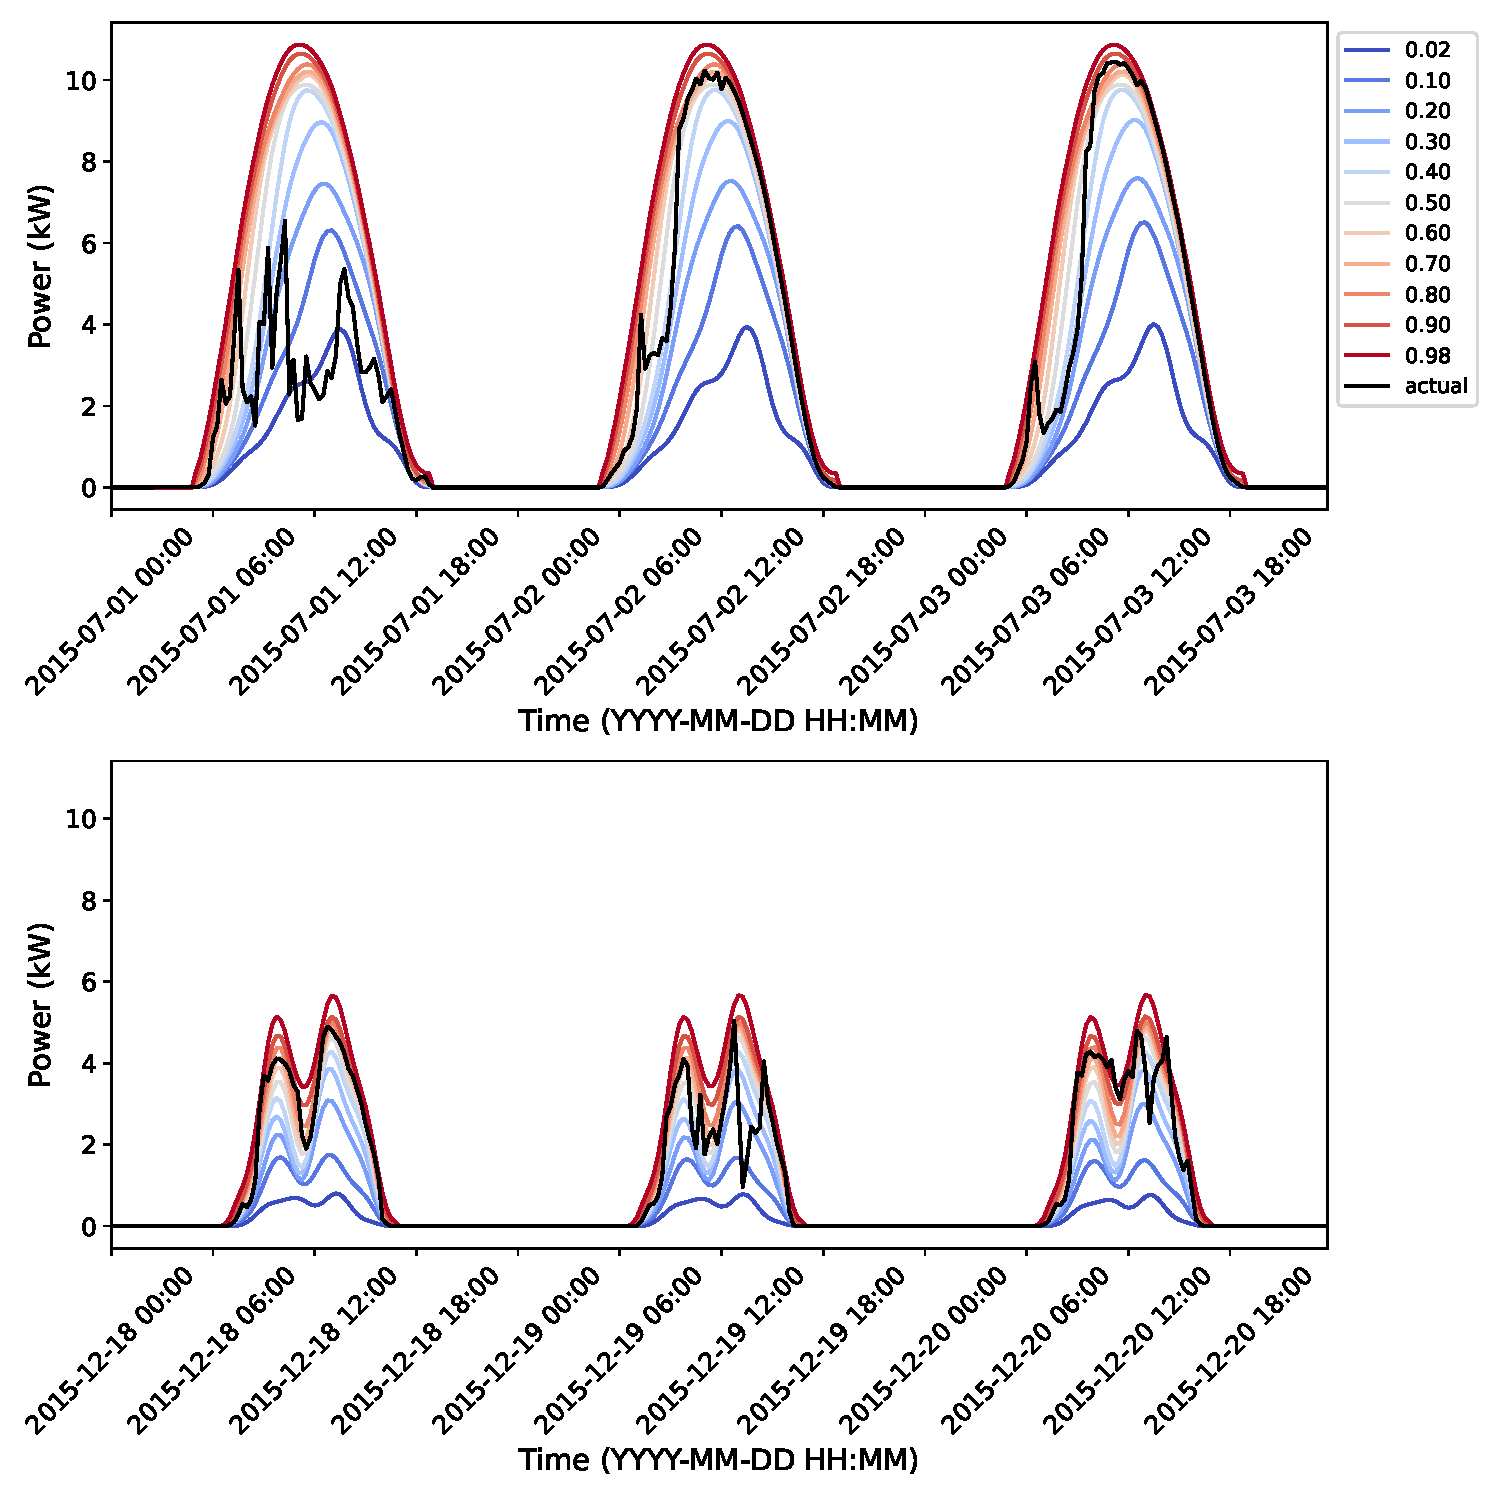
\includegraphics[width=\columnwidth]{./figures/quantiles_mapped_back.pdf}
		\end{figure}
	\end{column}
	\begin{column}{0.45\textwidth}
		\BIT
		\item estimating quantiles means estimating a probability distribution at each time
		\item can be done using quantile regression
		\item figure shows estimated quantiles for power generation of a residential PV system
		\EIT
	\end{column}
\end{columns}
\end{frame}

\begin{frame}{Model predictive control (MPC) for grid management}
\BIT
\item principled policy framework consisting of: \\
\hspace{12mm} $-$ \textbf{forecast:} predict stochastic future values \\
\hspace{12mm} $-$ \textbf{plan:} solve optimization problem assuming forecasts are correct \\
\hspace{12mm} $-$ \textbf{execute:} take first action in plan \\
\hspace{12mm} $-$ \textbf{repeat} 
\item works extremely well in practice (\eg \ to land rockets)
\item can be specified as a convex optimization problem
\item tractable and can be solved efficiently and robustly
\EIT
\end{frame}

\begin{frame}{Robust MPC}
\begin{columns}
	\begin{column}{0.65\textwidth}
		\begin{figure}
			\centering
			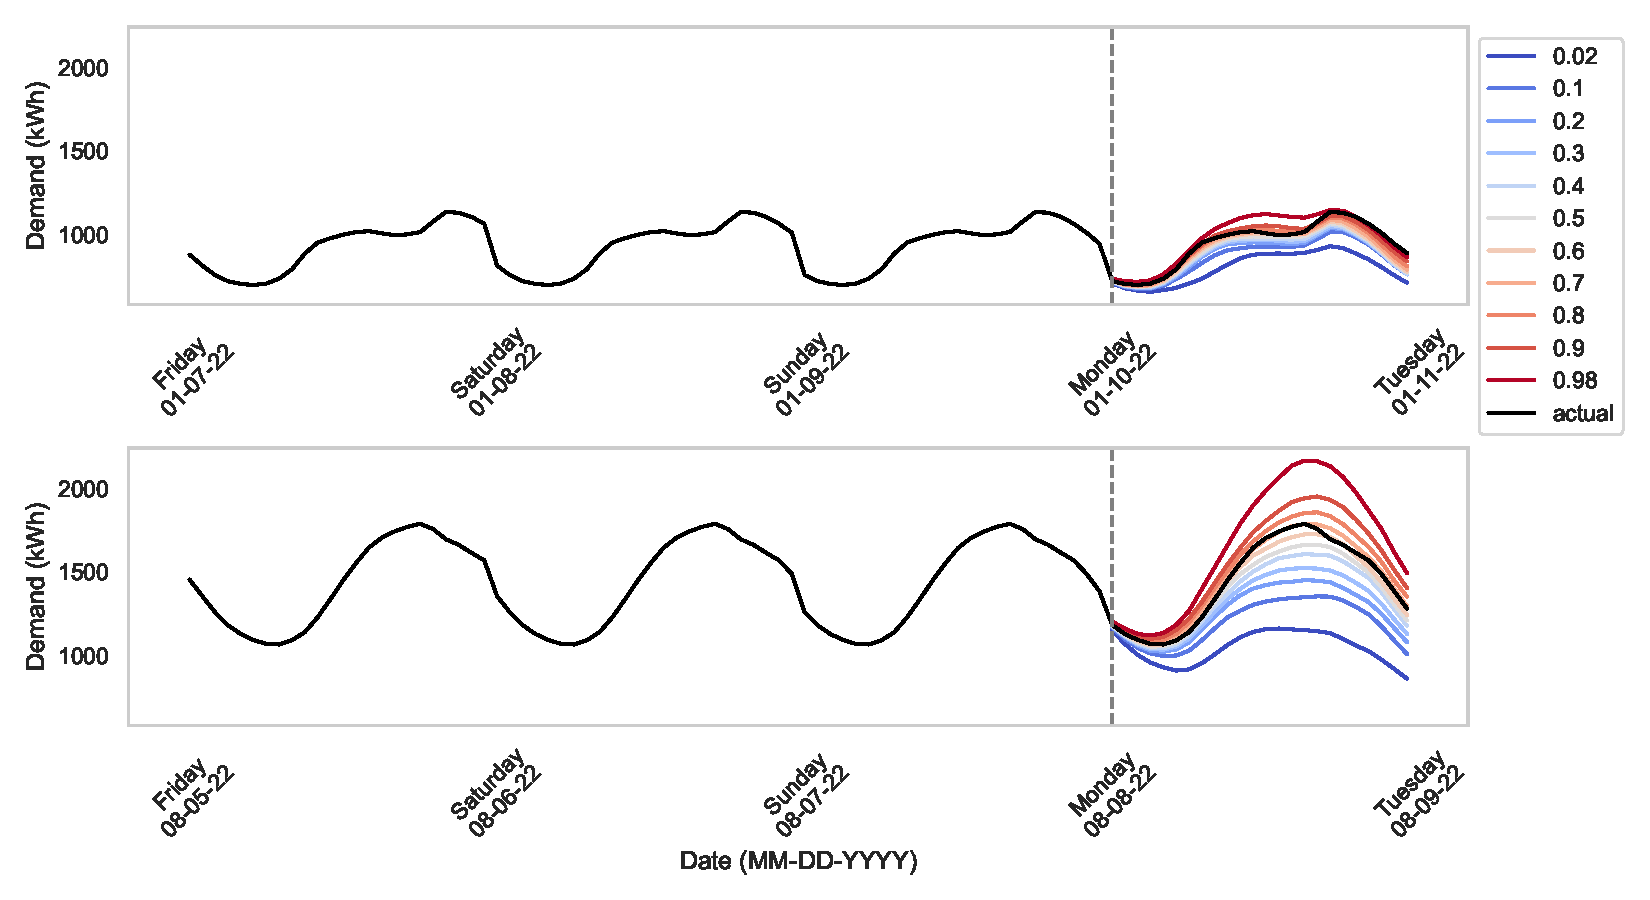
\includegraphics[width=\columnwidth]{./figures/marginal_quantile_forecasts.pdf}
		\end{figure}
	\end{column}
	\begin{column}{0.35\textwidth}
		\BIT
		\item figure shows quantile forecasts for net load in Rhode Island
		\item quantiles correspond to different risk levels
		\item can be tuned using historical data as well as future forecasts
		\EIT
	\end{column}
\end{columns}
\end{frame}

\begin{frame}{Prescient example}
\begin{columns}
	\begin{column}{0.65\textwidth}
		\begin{figure}
			\centering
			%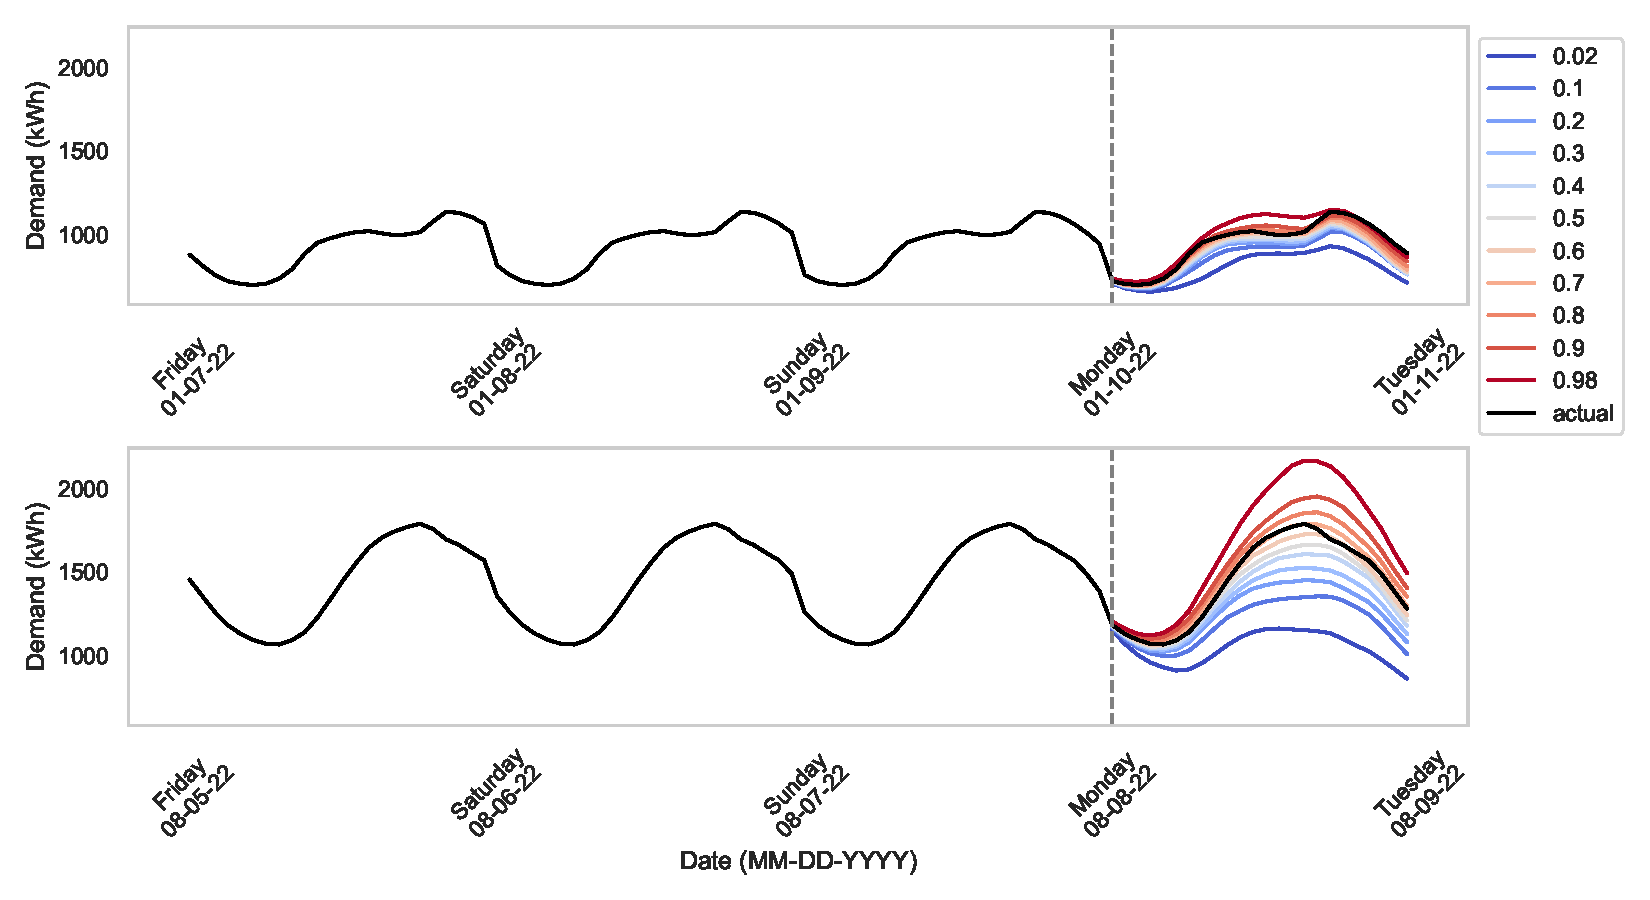
\includegraphics[width=\columnwidth]{./figures/marginal_quantile_forecasts.pdf}
		\end{figure}
	\end{column}
	\begin{column}{0.35\textwidth}
		\BIT
		\item start with a \textbf{prescient} model (full knowledge)
		\item provides a benchmark for MPC performance
		\item try causal model by replacing actual data with forecasts
		\item figure shows optimal charging policy for a battery
		\EIT
	\end{column}
\end{columns}
\end{frame}



	

\end{document}
